%This work is licensed under the Creative Commons Attribution-NonCommercial-NoDerivs 3.0 United States License. To view a copy of this license, visit http://creativecommons.org/licenses/by-nc-nd/3.0/us/ or send a letter to Creative Commons, 444 Castro Street, Suite 900, Mountain View, California, 94041, USA.

\section{Yb:KGW Laser System} \label{sec:laser}

% Draws from:
% High-power, femtosecond, thermal-lens-shaped Yb:KGW oscillator
% Joel A. Berger, Michael J. Greco, and W. Andreas Schroeder
% 9 June 2008 / Vol. 16, No. 12 / OPTICS EXPRESS

In order to experiment using very short laser pulses, we have designed and built a custom Ytterbium-doped potassium gadolinium tungstate (\ce{Yb$:$KGd(WO4)2} or Yb:KGW) laser system.\cite{berger_high-power_2008}
In practice, the flexibility afforded by having a custom-built system has outweighed its original performance benefit.
I have shown in Section \ref{sec:initial_conditions} that the electron pulse duration is not a simple function of the laser pulse duration, yet, at the time the laser was built, this fact was not yet obvious.
As such, our laser was designed to produce relatively high power output while generating ultrashort pulses, on the order of 250 fs for some conditions.

\subsection{Laser Introduction}
% page 8630
Yb:KGW is becoming a widely used solid-state gain medium for ultrafast laser systems.
As with other Yb-doped laser crystals \cite{Brenier_new_criteria}, this is primarily due to the gain medium's advantageous absorption properties for direct laser diode pumping at 980nm, its broad emission bandwidth around 1040nm, and consequent small ($\sim$ 6\%) quantum defect that results in a relatively low thermal load. 
Mode-locked (ML), diode-pumped, Yb:KGW laser oscillators generating pulses with sub-picosecond durations at average output powers in excess of 1W have been demonstrated \cite{Brunner_diode_pumped,Courjaud_high_power,Major_femtosecond_2006,Holtom_mode_locked_2006} and are now available commercially \cite{website_amplitude,website_solar}.
Such lasers have used dichroic mirrors \cite{Brunner_diode_pumped,Major_femtosecond_2006,Paunescu_diode_2004,Major_extended_2006}, polarization-coupling \cite{Holtom_mode_locked_2006}, or more complex optical geometries (e.g., thin disk lasers \cite{website_amplitude,Brunner_pulses_2002}) to pump the laser crystal in an efficient manner.

% page 8631
The spectroscopic properties of the biaxial Yb:KGW laser crystal \cite{Biswal_thermo_optical_05} indicate that the optimum diode pumping arrangement is for 980nm radiation polarized parallel to the optical $N_m$-axis since the crystal has the largest absorption cross-section in this configuration and, hence, the smallest absorption saturation intensity to drive the gain medium into a quasi 4-level system or to achieve transparency at the emission wavelength \cite{Brenier_new_criteria}.
However, as is the case for Yb-doped potassium yttrium tungstate (Yb:KYW) \cite{Liu_diode_pumped_2001,Killi_high_peak_2005}, mode-locked Yb:KGW lasers should ideally oscillate with radiation polarized parallel to the optical $N_p$-axis to access the broadest gain bandwidth around 1040nm, where the emission cross-section is comparable to that along the optical $N_m$-axis \cite{Holtom_mode_locked_2006,Biswal_thermo_optical_05}. This optimal requirement for orthogonal linear pump and laser polarizations led Holtom \cite{Holtom_mode_locked_2006} to employ a polarization-coupling scheme to diode pump longitudinally a 10W, sub-500fs, Yb:KGW laser.

%TODO is this first sentance correct or should I use "I" voice?
In this chapter, a high-power, femtosecond Yb:KGW oscillator is presented that also accesses the broader emission bandwidth parallel to the optical $N_p$-axis (parallel to the crystallographic $b$-axis), yet employs a simpler geometry for polarized diode-pumping on the strongest 980nm absorption line parallel to the optical $N_m$-axis (rotated by $\sim\,20^\circ$ from the crystallographic $a$-axis \cite{Biswal_thermo_optical_05,mochalov_laser_1997,pujol_crystalline_1999}).
The laser head design is based on the thermal lens shaping (TLS) technique developed in-house for astigmatism compensation in diode-pumped Nd-doped lasers with Brewster-cut gain media \cite{Rimington_thermal_lens_2004}.
It employs a simple single layer \ce{SiO2} anti-reflection coating on the gain medium to provide minimal loss for $p$-polarized intracavity 1040nm laser radiation and less than 0.5\% surface reflection for orthogonal $s$-polarized 980nm pump light.
The result is a simple and robust, soliton mode-locked and directly diode-pumped, solid-state laser oscillator delivering over 4W of average output power in a 63MHz train of pulses with a duration less than 300fs.
Frequency doubling of this laser output in a 2mm Brewster-cut Lithium triborate (LBO) crystal provides 1.65W of average power at 520nm.

The Watt-level green output power from the frequency-doubled sub-picosecond Yb:KGW oscillator corresponds to a visible peak laser pulse power in excess of 100kW, which is well-suited for further frequency conversion through harmonic generation or pumping of an ultrashort pulse optical parametric oscillator.
%TODO change voice/check ->
To our knowledge, the generation of subpicosecond green peak pulse powers greater than 100kW by frequency doubling the output of a laser oscillator has only been demonstrated for high-power thin-disk \cite{Brunner_powerful_2004,Marchese_pulse_energy_06} and cavity-dumped \cite{Palmer_microjoule_07} Yb-doped solid-state lasers, although externally-doubled commercial Ytterbium femtosecond oscillators \cite{website_amplitude,website_solar,website_high_q,website_time_bandwidth} and oscillators with rod-like Yb-fiber gain media \cite{Ortac_pulse_2007} can be expected to yield comparable peak green pulse powers.
%TODO replace to "This output will then be use to ..." and link to something from previous
%In our case, the visible femtosecond pulses will be used as the driving laser radiation source for an ultrafast electron microscope \cite{king_ultrafast_2005} --- a technology that seeks to combine the sub-nanometer spatial resolution of electron microscopy with the sub-picosecond temporal resolution afforded by today's ultrashort pulse laser systems.
%Critical to this technology is likely to be the development of a femtosecond photo-electron gun with a low spatial emittance \cite{zawadzka_evanescent_2001}.
%The coherent control of photoemission through visible laser-driven plasmon excitations on large-area (a few mm2), gold or silver, nano-patterned photocathodes may provide a mechanism by which this can be achieved \cite{zawadzka_evanescent_2001}.

\subsection{Laser Head Design}

The design of the laser head follows the example of Holtom \cite{Holtom_mode_locked_2006}, which ensures efficient pumping and access to the broadest emission bandwidth of Yb:KGW, while also employing the thermal lens shaping (TLS) technique to compensate for astigmatism \cite{Rimington_thermal_lens_2004}.
To ensure efficient operation of a Yb:KGW laser, the dominant absorption feature at 980nm for radiation polarized parallel to the optical $N_m$-axis ($\sim\,20^\circ$ from the crystallographic a-axis) should be pumped using high brightness diode lasers.
On the other hand, as with \ce{Yb$:$KY(WO4)2} \cite{Liu_diode_pumped_2001,Killi_high_peak_2005}, the broadest emission bandwidth for ultrashort pulse generation occurs for radiation polarized parallel to the optical $N_p$-axis (parallel to the crystallographic $b$-axis \cite{Holtom_mode_locked_2006}) in this biaxial material. 
%page 8632
Instead of using a polarization-coupled pumping geometry \cite{Holtom_mode_locked_2006} to ensure these optimum pump-lasing conditions, we employ the non-Brewster crystal geometry and cut shown in \ref{fig:crystal}\subref{fig:crystal_geo}, where a single 193nm-thick \ce{SiO2} anti-reflection coating is applied to both polished 3x10mm Yb:KGW crystal faces.
At an angle of incidence of 32.3$^\circ$, this coating theoretically has zero reflection loss for $p$-polarized 1040nm laser radiation parallel to the $b$-axis propagating perpendicular to the $a$-$b$ plane of the crystal (\ref{fig:crystal}\subref{fig:crystal_coating}); i.e., the preferred optical $N_p$-axis with refractive index $n_p$ = 1.98 \cite{Biswal_thermo_optical_05,pujol_crystalline_1999}.
The \ce{SiO2} coating also has an appropriate bandwidth for femtosecond laser operation in excess of 100nm (to the
0.1\% reflection points) for $p$-polarized radiation centered at 1040nm.
On the other hand, the $\sim$ 0.4\% reflection loss per surface for $s$-polarized 1040nm radiation is sufficient to suppress $s$-polarized oscillation in a laser resonator.
In addition, the same anti-reflection coating has less than 0.5\% reflection loss for $s$-polarized 980nm pump radiation (polarized parallel to the $a$-axis of the Yb:KGW crystal) at incidence angles between 21 and 39$^\circ$ (\ref{fig:crystal}\subref{fig:crystal_coating}).
Thus, in this Yb:KGW laser crystal geometry, the largest absorption cross-section associated with the optical $N_m$-axis is accessed with about 94\% efficiency ($\cos 20^\circ = 0.94$) by the $s$-polarized pump radiation.

\begin{figure}
  \subfloat[][]{
    \label{fig:crystal_geo}
    \begin{tikzpicture}
  % crystal
  \draw [thick,fill=white]
    (0,0) node [circle] (crystal1) {}
    -- ++(57.7:5)
      coordinate [pos=0.5] (beam in)
      node [pos=1,circle] (crystal2) {}
    -- ++(-32.3:1.5)
      node [circle] (crystal3) {}
    -- ++(237.7:5)
      node [circle] (crystal4) {}
    -- cycle
  ;
  % dimension
  \coordinate (longdim1) at ($(crystal1)+(147.7:0.4)$);
  \coordinate (longdim2) at ($(crystal2)+(147.7:0.4)$);
  \coordinate (shortdim1) at ($(crystal2)+(57.7:0.4)$);
  \coordinate (shortdim2) at ($(crystal3)+(57.7:0.4)$);
  \draw [thick,<->]
    (longdim1)
    -- (longdim2)
    node [pos=0.8,above left] {10cm} 
  ;
  \draw [thick,<->]
    (shortdim1)
    -- (shortdim2)
    node [pos=0.5,above right] {3cm} 
  ;
  % coating
  \begin{pgfonlayer}{background}
    \draw [fill=red]
      (crystal1.120)
      -- (crystal2.180)
      -- (crystal3.300)
        node [right,align=left] {193nm \ce{SiO2}\\AR coating} 
      -- (crystal4.0)
      -- cycle
    ;
  \end{pgfonlayer}
  % normal
  \draw [dashed]
    (beam in)
    -- +(147.7:1.5)
    -- +(147.7:-0.5)
  ;
  % beam
  \coordinate (beam start) at ($(beam in) - (2,0)$);
  \draw [very thick, ->, name path=beam]
    (beam start)
    -- (beam in)
    -- ++(-15.7:1.59)
    -- ++(2,0)
      coordinate [pos=0.6] (polarization)
  ;
  \draw [thick,<->]
    ($(polarization)+(0,0.3)$)
    -- ++(0,-0.6)
      node [align=left,below right] {1040nm laser\\radiation\\($p$-polarized)}
  ;
  % input angle marker
  \draw
    ($(beam in)!1cm!(beam start)$)
      node [above left] {$32.3^\circ$}
    arc [start angle=180, end angle=147.7, radius=1cm]
  ;
  % coord axes
  \node [draw,blue,circle,inner sep=3pt, right=0.5 of crystal1] 
    (axes) {}
  ;
  \node [draw,blue,fill,circle,inner sep=1.5pt]
    at (axes.center) {}
  ;
  \draw [blue,thick,->] 
    (axes)
      node [left] {$y$}
    -- ++(74.3:0.7)
      node [left] {$x$}
  ;
  % crystal axes
  \node [draw,circle,inner sep=3pt]
    at (crystal4) 
    (craxes) {}
  ;
  \node [draw,fill,circle,inner sep=1.5pt]
    at (craxes.center) {}
  ;
  \draw [very thick,dashed,->,name path=cryaxis] 
    (craxes)
      node [left] {$a$-axis}
    -- ++(74.3:3.5)
      node [right] {$b$-axis}
  ;
  % internal angle marker
  \draw 
    ($(crystal4)!1.5cm!(crystal3)$)
    arc [start angle=57.7, end angle=73.4, radius=1.5cm]
      node [pin={290:{$15.7^\circ$}}] {}
  ;
  % right angle
  \draw [name intersections={of=beam and cryaxis,by={int}}]
    ($(int)+(74.3:0.2)$)
    -- ++(-15.7:0.2)
    -- ++(74.3:-0.2)
  ;
\end{tikzpicture}


  }
  \subfloat[][]{
    \label{fig:crystal_coating}
    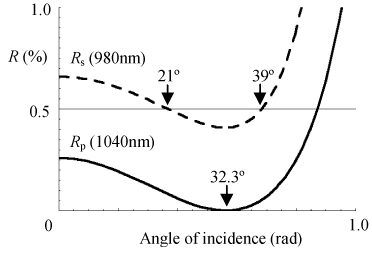
\includegraphics{coating.jpg}
  }
  \caption[Laser crystal and anti-reflection coating]{
    \protect\subref{fig:crystal_geo} Top view of the 3x3x10mm AR coated Yb:KGW laser crystal showing the crystal cut, the direction of propagation of p-polarized laser radiation at 1040nm, and the $x$ (tangential) and $y$ (saggital) directions (in blue) employed in the thermal analysis;
    \protect\subref{fig:crystal_coating} Calculated reflectivity of the 193nm \ce{SiO2} AR coating as a function of incidence angle for $p$-polarized 1040nm laser radiation (solid line) and $s$-polarized 980nm pump radiation (dashed line).
  }
  \label{fig:crystal}
\end{figure}

Efficient pumping is achieved with two, 35W, dual-axis collimated and TM-polarized laser diode arrays operating at 980nm (HLU35C10x5-980 from LIMO GmbH \cite{website_limo}).
The $\sim$3nm emission linewidth of the two laser diode arrays is well matched to the 3.7nm full-width half-maximum (FWHM) 980nm absorption line of Yb:KGW \cite{Paunescu_diode_2004,Biswal_thermo_optical_05,website_EKSPLA}.
Moreover, the two dual-axis collimated laser diodes have full-angle $1/e^2$ intensity beam divergences of $\theta_y \approx$ 4.4mrad and $\theta_x \approx$ 6.8mrad in the horizontal ($x$-direction parallel to the emitter array) and vertical ($y$) directions respectively. 
With 100mm focal length lenses, this allows the pump radiation to be focused to a pump spot diameter 2W $\approx$ 400$\mu$m, yielding a maximum incident pump irradiance of $\sim$28kW/cm$^2$ from one laser diode array.
The Yb concentration was chosen to be 2\% atomic doping to ensure that more than 90\% of the pump radiation was absorbed over the 3mm Yb:KGW crystal thickness.
With the employed counter-propagating pump geometry, the resultant maximum average pump irradiance over the crystal length is then roughly 3 times the $\sim$6kW/cm$^2$ saturation intensity of the dominant 980nm absorption line \cite{Brunner_powerful_2004}.
The laser crystal was obtained from NovaPhase \cite{website_nova}.

To ensure a stigmatic laser resonator, we also employ the thermal lens shaping (TLS) technique \cite{Rimington_thermal_lens_2004} to compensate for the astigmatism induced by the non-normal incidence geometry of the laser crystal. 
For the employed non-Brewster crystal cut (\ref{fig:crystal}\subref{fig:crystal_geo}), a ray
%page 8633
transfer matrix analysis (with the $x$ direction parallel to the crystallographic $b$-axis and the $y$
direction parallel to the $a$-axis) reveals that the required ellipticity for a stigmatic thermal lens
generated by a parabolic temperature distribution, $T(x, y) = T_0 - \frac{1}{2} ( A_\smallT x^2 + B_\smallT y^2 )$, where $T_0$
is the on-axis temperature, is given by
%TODO check W symbol consistent with the rest of the paper
\begin{equation} \label{eq:laser_ratio_ba}
  \frac{B_\smallT}{A_\smallT} = 
  \frac{ \cos^2 \theta_2 \left( \dfrac{dn}{dT} \right) + 2 \Delta \alpha_\smallT \left( n \cos\theta_2 - \cos\theta_1 \right) }
       { \cos^2 \theta_1 \left[ \left( \dfrac{dn}{dT} \right) + 2 \Delta \alpha_\smallT \left( n \cos\theta_2 - \cos\theta_1 \right) \right] }
  \quad\text{.}
\end{equation}
Here, $\frac{dn}{dT}$ and $n$ are the thermo-optic coefficient and refractive index of the medium respectively (in this case for radiation polarized along the optical $N_p$-axis), $\theta_1$ is the 32.3$^\circ$ angle of incidence, $\theta_2$ = 15.7$^\circ$ is the angle of refraction (as $n_p$ = 1.98 \cite{Biswal_thermo_optical_05,pujol_crystalline_1999}), and $\Delta$ is the fraction of the crystal length $l$ contributing to the bowing of the crystal faces under thermal
expansion with coefficient $\alpha T$ \cite{Rimington_thermal_lens_2004}.
Generally, $\Delta \approx W l$ , where $W$ is the transverse size (radius) of the pumped region \cite{Koechner_thermal_1970}.
In our case, $l \approx$ 3mm and $W \approx$ 0.2mm, so that $\Delta < 0.1$, implying that the thermal duct due to a non-zero $\frac{dn}{dT}$ primarily determines the required $B_T$/$A_T$ ratio.
In other words, for the potassium gadolinium tungstate (\ce{KGd(WO4)2}) crystal geometry of \ref{fig:crystal}\subref{fig:crystal_geo}, we expect from \ref{eq:laser_ratio_ba} to require $\dfrac{B_\smallT}{A_\smallT} \approx \dfrac{ \cos^2 \theta_2 }{ \cos^2 \theta_1 } = 1.3$.

The spatial pump distribution needed to generate the required $B_T/A_T$ ratio can be found using a cosine Fourier series solution to the thermal diffusion equation for our two-dimensional problem,
\begin{equation} \label{eq:heat_eqn}
  \kappa \nabla^2 T(x,y) = Q(x,y)
  \quad\text{,}
\end{equation}
where $\kappa$ is the thermal diffusion coefficient.
Thermal diffusion in the third $z$-direction has been neglected due to the relatively uniform longitudinal heat deposition resulting from our counter-propagating pump geometry \cite{Rimington_thermal_lens_2004}.
The specifications of our dual-axis collimated diodes \cite{website_limo} indicate that heat source can be represented mathematically as
\begin{equation}
  Q(x,y) = Q_0 \exp \left[ - \frac{x^2}{W_x^2} - \left( \frac{y^2}{W_y^2} \right)^3 \right]
  \quad\text{;}
\end{equation}
that is, the focused pump radiation is described accurately by a Gaussian irradiance distribution in the horizontal ($x$) direction with half-width 1/e maximum (HW1/eM) spot size $W_x$ and a super-Gaussian of order 3 in the vertical ($y$) direction with spot size $W_y$.
\ref{eq:heat_eqn} can then be solved using the appropriate boundary conditions for our 3x10mm crystal cross-section for the employed TLS technique \cite{Rimington_thermal_lens_2004}; namely, heat removal only through the top crystal face implies $T(x,y = \pm 1.5\text{mm}) = 0$ (or arbitrary constant) and $\dfrac{\partial T}{\partial x} = 0$ at $ x = \pm 5.0$mm for any $y$.
For a fixed vertical pump spot size of $W_y = 0.2$mm, our analysis indicates that in order to achieve the required ratio $B_T / A_T = 1.3$ in the parabolic approximation for $T(x,y)$ about $(x,y) = (0,0)$ a horizontal pump spot size $W_x = 0.3$mm is needed; in other words, the required $Q(x,y)$ heat source spot size ratio (or ellipticity) $W_x / W_y = 1.5$.
This analytical result for the central region around the laser beam axis is shown in \ref{fig:laser-thermal}; displayed are the
%page 8634
horizontal ($y = 0$, \ref{fig:laser-thermal}(a)) and vertical ($x = 0$, \ref{fig:laser-thermal}(b)) sections, respectively, through the $Q(x,y)$ and $T(x,y)$ distributions.
Also shown are the parabolic approximations to the pump-induced temperature distribution (dashed lines) and representative TEM$_{00}$ Gaussian laser modes (shaded area) in the Yb:KGW crystal with a HW1/eM field mode sizes of $w_y = 160\mu$m and $w_x = 182 \mu$m (14\% larger due to refraction (\ref{fig:crystal}\subref{fig:crystal_geo}).
This mode size ensures efficient pump-probe overlap while minimizing the loss due to ground state absorption in the unpumped regions of the Yb-doped gain medium \cite{Brenier_new_criteria}; in particular, in the vertical direction (\ref{fig:laser-thermal}(b)) where $w_y$ greater than about $0.8 W_y$ leads to significant absorptive loss as the extrema of the laser mode extend beyond the sharply-bounded super-Gaussian pump region.

\begin{figure}
  \centering
  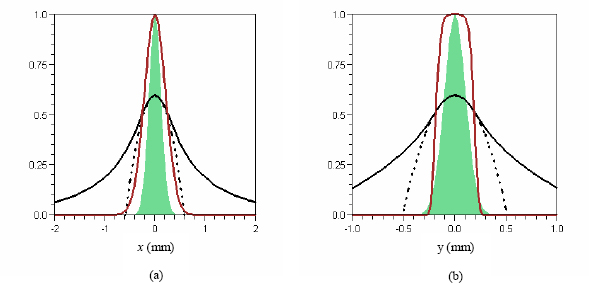
\includegraphics{thermal.jpg}
  \caption[Thermal profile and thermal lens shaping of KGW crystal pumping]{
    Analytical evaluation of the temperature distribution $T(x,y)$ due to the Gaussian/super-Gaussian heat source $Q(x,y)$ in the (a) horizontal ($y=0$) and (b) vertical ($x=0$) directions: $Q(x,y)$ - red-brown line; $T(x,y)$ - black line; parabolic approximation to $T(x,y)$ - dashed black line; representative TEM$_{00}$ laser field modes - solid green.
  }
  \label{fig:laser-thermal}
\end{figure}

The analysis clearly shows that the TEM$_{00}$ laser mode will experience a near perfect pump-induced thermal lens upon propagation through the gain medium --- the deviation of $T(x,y)$ from the parabolic approximation, and hence a perfect dominant thermo-optic (GRIN) duct, being insignificant over the size of the laser mode in both the horizontal and vertical directions.
Moreover, the fact that $W_x \approx 1.6 w_x$ implies that some degree of horizontal spatial walk-off between the pump and laser beams can be tolerated in this TLS geometry.
For example, when the pump and laser beams are exactly overlapped at the center of the Yb:KGW crystal, an external angle of 0.1rad (= 5.7$^\circ$) would generate an effective spatial walk-off of only about 75$\mu$m over our 3mm gain crystal length.
Clearly, this can be readily accommodated by the $W_x = 0.3$mm horizontal pump spot size when $w_x \approx 180\mu$m.
However, even though $W_x > w_x$, the Gaussian (rather than super-Gaussian) horizontal pump mode profile is still expected to assist in ensuring TEM$_{00}$-mode operation since the net horizontal gain profile (gain minus absorptive loss) will fall off more rapidly than the pump profile for a quasi-three level Yb-doped gain medium \cite{Brenier_new_criteria}.

We note that the above thermal lens analysis neglects the anisotropy of the thermal conductivity $\kappa$ in potassium gadolinium tungstate (\ce{KGd(WO4)2}) \cite{Biswal_thermo_optical_05,mochalov_laser_1997} and stress-induced refractive index changes \cite{Yumashev_laser_2007}.
For the employed crystal cut in our TLS geometry (\ref{fig:crystal}\subref{fig:crystal_geo}), the anisotropy in $\kappa$ \cite{mochalov_laser_1997,website_EKSPLA} is not expected to have a significant effect; the laser head geometry dictates that the dominant pump-induced heat conduction will be in the saggital ($y$) direction along the crystal $a$-axis where $\kappa \approx 2.6$W/(mK) (heat extraction only through the top and bottom 3x10mm crystal faces), so that the 46\% larger value of $\kappa$ along the $b$-axis ($x$) direction at 3.8W/(mK) should not have a large influence on the heat conduction.
The refractive index
%page 8635
changes due to stress in the pumped gain medium are difficult to quantify since the substantial variations in the reported values of the thermo-optic coefficients in KGW make it impossible to extract either the sign or magnitude of the stress dependence of the refractive index \cite{website_time_bandwidth}.
Moreover, nearly all analyses of thermal lensing effects Nd:KGW and Yb:KGW lasers have been performed for laser radiation polarized along the optical $N_m$-axis, which accesses the largest emission cross-section for both Nd- and Yb-doping \cite{Yumashev_laser_2007,Hellstrom_efficient_2006}.
Consequently, for our laser polarized along the optical $N_p$-axis \cite{Holtom_mode_locked_2006}, there is insufficient information to include accurately the effects of stress-induced refractive index changes.

\subsection{The Yb:KGW laser cavity}

The diode-pumped TLS Yb:KGW laser head is placed in the 2.35m-long, asymmetric z-fold cavity shown in \ref{fig:laser-cavity}\subref{fig:laser_schematic}.
The two focusing gain section mirrors each have a group velocity dispersion (GVD) of $-1300 ( \pm 150 ) \text{fs}^2$ (Layertec GmbH \cite{website_layertec}), a radius of curvature $R$ = 50cm, and are positioned 29.5cm from the gain medium.
The 5$^\circ$ angle of incidence on the gain section mirrors results in minimal astigmatism, although any net round-trip cavity astigmatism can be compensated for by the TLS technique.
The longer 75cm arm of the resonator is terminated by a concave ($R$ = 1m and angle of incidence $< 2^\circ$) high reflector
%page 8636
focusing the intracavity radiation on a saturable Bragg reflector (SBR) with a 1\% reflectivity modulation depth at 1040nm (BATOP GmbH \cite{website_BATOP}) positioned a distance $z$ from the focusing mirror.
The shorter 63cm arm is terminated by a plane output coupler with a 7\% transmission at 1040nm.
As a free-running oscillator (SBR focusing section replaced by flat high reflector at $d_2$ = 75cm), the laser produced over 6W of TEM$_{00}$ ($M^2 < 1.2$) output power.

\begin{figure}
  \centering
  \subfloat[][]{
    \label{fig:laser_schematic}
    %This work is licensed under the Creative Commons Attribution-NonCommercial-NoDerivs 3.0 United States License. To view a copy of this license, visit http://creativecommons.org/licenses/by-nc-nd/3.0/us/ or send a letter to Creative Commons, 444 Castro Street, Suite 900, Mountain View, California, 94041, USA.

\begin{tikzpicture}
  % laser crystal
  \draw [thick, fill=red!80]
    (0,0) 
    -- ++(-32.3:3mm)
    -- ++(-122.3:10mm)
      coordinate [pos=0.47] (crystal right)
    -- ++(147.7:3mm)
      node [pos=0,below] {Yb:KGW}
    -- ++(57.7:10mm)
      coordinate [pos=0.47] (crystal left)
    -- cycle
  ;
  % beam path in crystal
  \draw [very thick] (crystal left) -- (crystal right);

  % pump lasers
  \node [left=3 of crystal left, fill=yellow, draw] (LD left) {LD};
  \draw [orange, ultra thick, -latex]
    (LD left)
    -- (crystal left)
      coordinate [pos=0.2] (LD lens left)
  ;
  \node [
      draw,
      shape=ellipse,
      inner xsep=0.5mm,
      inner ysep=3mm,
      fill=blue!30,
      label={above:$f=$100mm}
    ]
    at (LD lens left) {};
  \node [right=3 of crystal right, fill=yellow, draw] (LD right) {LD};
  \draw [orange, ultra thick, -latex]
    (LD right)
    -- (crystal right)
      coordinate [pos=0.2] (LD lens right)
  ;
  \node [
      draw,
      shape=ellipse,
      inner xsep=0.5mm,
      inner ysep=3mm,
      fill=blue!30,
      label={below:$f=$100mm}
    ]
    at (LD lens right) {};

  % laser top branch
  \coordinate [above=6mm of LD right] (top turning mirror);
  \draw [very thick]
    (crystal right)
    -- (top turning mirror)
    -- ++(177:8)
      node [pos=0.5,above] {$d_1=$63cm}
      coordinate [pos=1] (OC)
  ;
  \draw [
      fill=blue!30,
    ]
    ($(top turning mirror)+(-0.5mm, 2.5mm)$)
    .. controls ($(top turning mirror)+(3:0.5mm)$)
      .. ++(273:5mm)
    -- ++(3:2mm)
    -- ++(93:5mm)
      node [above right,align=left] {$R=$50cm\\GVD=-1300fs$^2$}
    -- cycle
  ;
  \node [
      draw,
      rectangle,
      inner xsep=1mm,
      inner ysep=3mm,
      fill=blue!30,
      rotate=-3,
      label={below:OC}
    ] 
    at (OC) {}
  ;
  \node [
    draw,
    fill=purple,
    shape=single arrow,
    left=3mm of OC,
    shape border rotate=180,
    single arrow head extend=1.2mm,
    inner xsep=3mm,
    inner ysep=0.5mm,
    rotate=-3
  ] {};

  % laser bottom branch
  \coordinate [below=6mm of LD left] (bottom turning mirror);
  \draw [very thick]
    (crystal left)
    -- (bottom turning mirror)
    -- ++(-3:9)
      node [pos=0.5,below] {$d_2=$75cm}
      coordinate [pos=1] (extension turning mirror)
    -- ++(183:3)
      node [pos=0.5,below] {$z$}
      coordinate [pos=1] (SBR)
  ;
  \draw [
      fill=blue!30,
    ]
    ($(bottom turning mirror)+(0.5mm, 2.5mm)$)
    .. controls ($(bottom turning mirror)+(3:-0.5mm)$)
      .. ++(273:5mm)
    -- ++(3:-2mm)
      node [below,align=left] {$R=$50cm\\GVD=-1300fs$^2$}
    -- ++(93:5mm)
    -- cycle
  ;
  \draw [
      fill=blue!30,
    ]
    ($(extension turning mirror)+(-0.5mm, 2.5mm)$)
    .. controls ($(extension turning mirror)+(3:0.5mm)$)
      .. ++(273:5mm)
    -- ++(3:2mm)
      node [below] {$R=$100cm}
    -- ++(93:5mm)
    -- cycle
  ;

  % SBR
  \node [fill=black,rotate=3,inner xsep=0.5mm] at (SBR) {};
  \node [draw, rotate=3,inner ysep=3mm] at ($(SBR)+(183:1.7mm)+(273:1.8mm)$) {};
  \node [below=5mm of SBR] {SBR ($\Delta R=$ 1\%)};
  
\end{tikzpicture}


  }
  \\
  \subfloat[][]{
    \label{fig:laser_stability}
    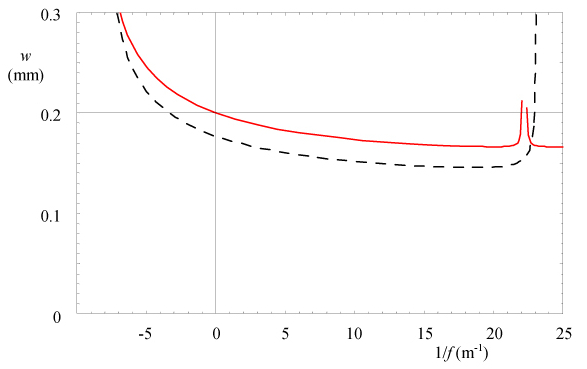
\includegraphics{stability.jpg}
  }
  \caption[Schematic and stability plot of employed Yb:KGW ultrafast laser]{
    \protect\subref{fig:laser_schematic} Schematic of the femtosecond TLS Yb:KGW oscillator (LD = laser diode, OC = output coupler, SBR = saturable Bragg reflector).
    \protect\subref{fig:laser_stability} Laser mode size in the center of the Yb:KGW gain medium ($w$) as a function of the strength of the lensing ($1/f$) in the gain medium (thermal and Kerr) obtained from a resonator stability analysis with $z \approx 42$cm for both the tangential ($x$, red line) and saggital ($y$, dashed black line) directions.
    The 0.2mm (HW1/eM) vertical super-Gaussian pump spot size is indicated by the horizontal line.
  }
  \label{fig:laser-cavity}
\end{figure}

The stability analysis of our diode-pumped Yb:KGW laser (\ref{fig:laser-cavity}\subref{fig:laser_stability}), clearly indicates that the resonator configuration is unstable for thermal focal lengths less than about $-6m^{-1}$ (diopters) and is unlikely to oscillate for negative thermal focal lengths as this requires a vertical TEM$_{00}$-mode size $w_y$ greater than 180$\mu$m in the Yb:KGW gain medium --- a value that would result in strong absorptive losses due to the restrictive $W_y = 200\mu$m super-Gaussian vertical pump beam size in the Yb-doped crystal.
The clear implication is therefore that the net thermal lens due to the dominant thermal duct is positive; that is, the sum of the refractive index change due to the thermo-optic coefficient and stress for 1040nm laser radiation polarized along the optical $N_p$-axis (crystal $b$-axis) is positive.
This result is in apparent contradiction to some recent measurements of relatively large negative thermo-optic coefficients in Yb:KGW \cite{Biswal_thermo_optical_05}, but is consistent with other determinations of the pump-induced thermal focal length for laser oscillation polarized parallel to the optical $N_p$-axis \cite{Holtom_mode_locked_2006,Hellstrom_efficient_2006}.

\subsection{Mode-locked laser operation}

In the cavity configuration depicted in \ref{fig:laser-cavity}\subref{fig:laser_schematic}, self-starting mode-locked (ML) operation was observed for output powers greater than $\sim$2W and $z \approx 42$cm.
The maximum (or optimum) mode-locked output power obtained without the emergence of DC spectral components was 3.5W, with a sech$^2$ pulse duration of 250fs (\ref{fig:laser-profile}(a)).
The insertion of two plane dispersion compensation mirrors each with a GVD of $-700\text{fs}^2$ (Layertec GmbH \cite{website_layertec}) into the short arm of the cavity generated higher mode-locked output powers with longer pulse durations.
For example, with two reflections off each mirror (an additional $-5600\text{fs}^2$ of round-trip GVD), the pulse duration increased to 347fs (\ref{fig:laser-profile}(b)) at an optimum mode-locked output power of $5.0$W.
This trend is consistent with the expected `soliton' modelocking regime; that is, the SBR only initiates the mode-locking mechanism, which is quickly dominated by self-phase modulation in the Yb:KGW gain medium balanced by the net negative GVD in the cavity \cite{Brunner_diode_pumped}.

\begin{figure}
  \centering
  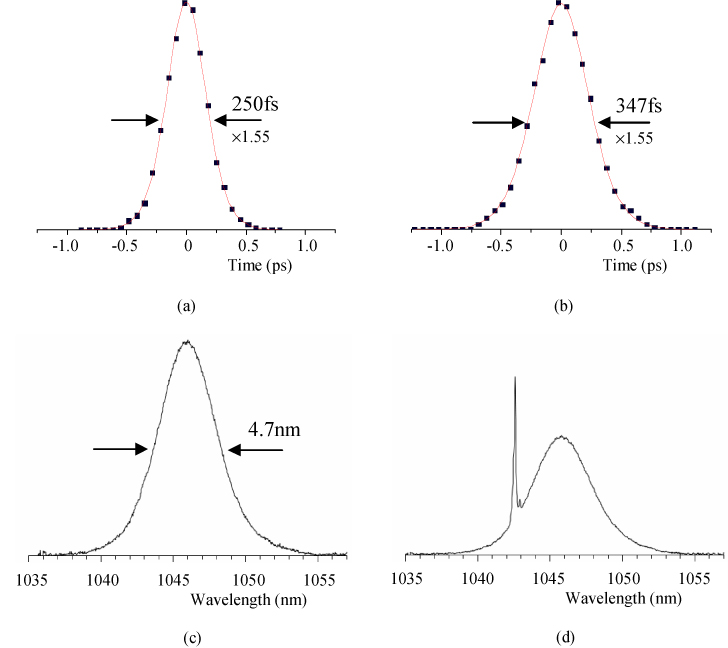
\includegraphics{profile.jpg}
  \caption[Autocorrelation measurements of employed ultrafast laser's pulse duration]{
Second harmonic autocorrelation measurements and output spectra of the ML Yb:KGW laser; (a) the 250fs laser pulse duration (and fit assuming a sech$^2$ pulse shape) for the cavity depicted in \protect\ref{fig:laser-cavity}\protect\subref{fig:laser_schematic} at an output power of 3.5W, (b) the 347fs pulse duration (and fit assuming a sech$^2$ pulse shape) obtained with an additional -5600fs$^2$ of round-trip GVD at an output power of 5W, (c) the 4.7nm full-width half maximum spectrum associated with the 250fs ML pulse of (a), and (d) spectral output for the ML resonator of \protect\ref{fig:laser-cavity}\protect\subref{fig:laser_schematic} at a laser power of 3.7W.
  }
  \label{fig:laser-profile}
\end{figure}

The laser is capable of generating shorter ML pulse durations.
Replacement of one of the $-1300 ( \pm 150 ) \text{fs}^2$ z-fold mirrors with a conventional $R = 50$cm high reflector and the insertion of $-880\text{fs}^2$ of negative GVD per round trip (a pair of $-220\text{fs}^2$ dispersion compensating mirrors) generated $\sim220$fs pulses at 24A of diode current, 2W of output power, and a SBR position $z = 43.2$cm.
However, ML operation was significantly less stable under these conditions, indicating that either the cavity is operating close to the net zero GVD point or that the finite gain bandwidth is influencing the ML operation.
We also note that in this case the optimum SBR position $z$ is larger than that for higher power 3.5W ML operation with a negative cavity GVD of $-5,200\text{fs}^2$ per round-trip \ref{fig:laser-profile}(a)), but is always less than the 50cm focal length of the concave high reflector.
This is due to the need to match the absorption-induced thermal bowing of the SBR (i.e., the radius of curvature of its front surface mirror) to the radius of curvature of the intra-cavity laser mode \cite{Schieffer_dual_passive_2006}.
In general, good ML operation is achieved with the SBR positioned within $\pm$1cm from the optimum $z$ distance.

\ref{fig:laser-performance} shows the laser's output power as a function of diode current for the cavity configuration depicted in \ref{fig:laser-cavity}\subref{fig:laser_schematic}; a total negative GVD of $-5,200\text{fs}^2$ per round-trip and a 7\% transmission output coupler.
Soliton mode-locked (ML) operation is observed for diode currents greater than 23A, corresponding to a continuous-wave (CW) output power of 1.8W.
Between diode currents (output powers) of 23 and 25A (1.8 and 2.3W), the resonator operates mainly in the CW mode, but will transition to ML operation upon being subjected to a perturbation.
The switching to ML operation is accompanied by a 250mW increase in output
%page 8637
power indicating a higher cavity Q for ML operation.
This is consistent both with the laser accessing more of the available inhomogeneous gain bandwidth and with our resonator design favoring operation with a strong Kerr lens in the Yb:KGW gain medium.
Given a value of $n^2 \approx 15 \cdot 10^{-16}\text{cm}^2/\text{W}$ for 1040nm radiation polarized parallel to the KGW crystal's optical $N_p$-axis \cite{Major_characterization_2003,Selivanov_nonlinear_2006,Vodchits_zscan_2006} and a calculated peak pulse irradiance of $\sim$4GW/cm$^2$ in the gain medium at 24A, we expect a Kerr lens strength of approximately 2m$^-1$.
From \ref{fig:laser-cavity}\subref{fig:laser_stability}, we see that the resulting increase in the strength of the lensing in the Yb:KGW crystal will result in a reduction of the laser mode size in the gain medium, which produces a better spatial match to gain duct produced by the laser diode pumps (less absorptive loss), thus generating an increase in output power.

\begin{figure}
  \centering
  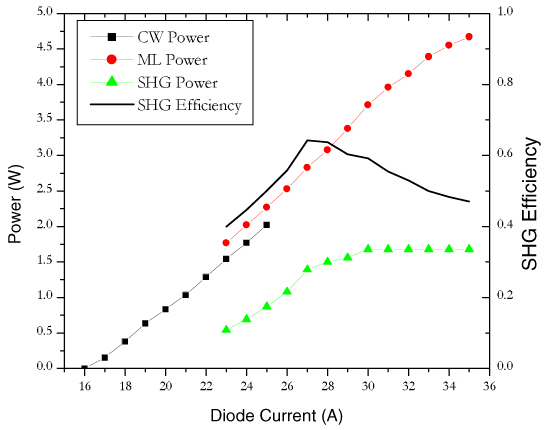
\includegraphics{performance.jpg}
  \caption[Power measuments of employed ultrast laser]{
Performance of the diode-pumped, TLS, Yb:KGW laser (in the cavity configuration of \protect\ref{fig:laser-cavity}\protect\subref{fig:laser_schematic} ) as a function of applied diode current: continuous-wave (CW) output power (black squares); mode locked (ML) output power (red circles); frequency doubled power (green triangles); and second harmonic generation (SHG) efficiency (line).
  }
  \label{fig:laser-performance}
\end{figure}

Above a diode current of 25A (i.e., an output power of 2.3W), the laser exhibits spontaneous self-starting ML operation.
At a diode current around 29A, a maximum (or optimum) average mode-locked output power of $\sim$3.5W is obtained.
The 250fs pulses generated at this output power (\ref{fig:laser-profile}(a)) correspond to a Kerr lens strength in the Yb:KGW crystal of $\sim4 \text{m}^{-1}$, which is readily accommodated by the resonator design (\ref{fig:laser-cavity}\subref{fig:laser_stability}).
For this $\sim$3.5W ML laser with a negative cavity GVD of $-5,200\text{fs}^2$ per round-trip, the full-width at
%page 8638
half maximum of the mode-locked spectrum centered at 1046nm is 4.7nm (\ref{fig:laser-profile}(c)).
The laser is therefore generates pulses with a time-bandwidth product very close to the Fourier limit of 0.32 for a sech$^2$ pulse shape.
At output powers greater than 3.5W, a DC spectral component emerges at the short wavelength end of the ML spectrum (\ref{fig:laser-profile}(d)) and there is a slow roll-over in the laser output power (\ref{fig:laser-performance}).
This trend is expected for a Yb:KGW soliton ML laser; in this case, the soliton power limit being reached at about 29A, and the asymmetric spectral gain of Yb:KGW forcing excess CW laser power oscillation at wavelengths shorter than the peak of the ML spectrum.
Similar laser performance is observed with the insertion of an additional $-5,600\text{fs}^2$ of cavity GVD per round trip, which generates 347fs sech$^2$ pulses (\ref{fig:laser-profile}(b)); that is, a DC spectral component appears on the short wavelength side of a narrower $\sim$3.5nm ML spectrum at output powers above 5W.

\subsection{Frequency doubling}

The ML output from the femtosecond Yb:KGW laser with a net negative GVD of $-5,200\text{fs}^2$ per round-trip was frequency doubled in a critically phase-matched, 2mm, Type I Lithium triborate (LBO) crystal.
The crystal is uncoated and cut for frequency doubling with the fundamental $p$-polarized radiation at 1046nm incident at Brewster's angle --- a geometry that ensures both minimum loss for the fundamental radiation and, more importantly, a high damage threshold.
The doubling crystal is positioned at the focus of a $z$-fold comprising a 1040nm high reflector with a radius of curvature of 75mm followed by a collimating mirror with a radius of curvature of 100mm reflective at both the fundamental and second harmonic wavelengths.
At the 3.5W ML output power, with a pulse duration of 250fs, the estimated focal irradiance for the fundamental is $\sim50\text{GW}/\text{cm}^2$ in the LBO doubling crystal.
Two plane dispersion compensation mirrors, each with a GVD of $-220\text{fs}^2$ (Layertec GmbH \cite{website_layertec}), inserted before the $z$-fold doubling geometry compensate for propagation through the 6mm-thick fused silica output coupler, reflections off standard optics, etc.
After the collimating
%page 8639
mirror, a standard flat dichroic beamsplitter then separates the reflected $s$-polarized 523nm radiation from the transmitted $p$-polarized fundamental.

This frequency doubling geometry for LBO is chosen to be close to the optimum for efficient short pulse doubling \cite{wang_efficiency_2003,Saltiel_second_harmonic_2004} defined by limits imposed by group-velocity walk-off between the fundamental and second harmonic pulses, spatial walk-off in the critical phase-matching, and the ratio of the confocal parameter of the focused fundamental wave to the LBO crystal length.
In addition, the $z$-fold configuration allows for astigmatism compensation (e.g., due to the Brewster LBO crystal) of the second harmonic output by adjustment of the angle of incidence on the second collimating mirror.

\ref{fig:laser-performance} shows the resultant frequency-doubled green power for the ML Yb:KGW laser.
The measured average power at 523nm increases rapidly from 0.5W at the 23A mode-locking threshold to over 1.3W at a diode drive current of 27A.
At and above 30A, the second harmonic power saturates at 1.65W --- an effect that is clearly consistent with the observed emergence of a DC spectral component at diode currents above 29A since only the ML pulse will be efficiently frequency doubled.
Also plotted in \ref{fig:laser-performance} is the frequency doubling efficiency, which is calculated taking into account the 17\% loss suffered by the $s$-polarized 523nm radiation upon exiting the Brewster-cut LBO crystal and the 4\% loss (to diagnostics) of the fundamental radiation prior to the $z$-fold doubling geometry.
The maximum doubling efficiency of over 60\% occurs at 27-28A of diode drive current when the ML laser output power is $\sim$3W.
At a ML output power of 3.5W (29-30A), the frequency doubling efficiency is still $\sim$60\% and slowly decreases above 30A as the DC spectral component absorbs the residual power above the soliton power limit.

\subsection{Summary}


A robust, high-power ($\sim$5W), diode-pumped and thermal-lens-shaped, femtosecond (220-350fs) Yb:KGW oscillator is presented.
The ML operation of the laser is self-starting above a critical output power of $\sim$2W, being initiated by a 1\% modulation depth SBR and subsequently supported in the soliton regime through a balance of self-phase modulation (Kerr lensing) in the gain medium and negative GVD (introduced using dispersion compensating mirrors).
The use of the TLS technique in the diode-pumped laser head provides for astigmatism-compensated TEM$_{00}$-mode operation (a spatial beam quality $M^2 <1.2$), while proper cavity design accommodates the strong Kerr lens (up to $\sim4\text{m}^{-1}$) in the Yb:KGW crystal under ML operation.
A full analysis of the thermal conduction in our 3x3x10mm Yb:KGW crystal is used to determine the correct TLS pump conditions, which lead to both excellent pump-laser beam overlap for the near collinear pump geometry and a near perfect pump-induced thermal lens (i.e., parabolic temperature distribution) experienced by the intracavity laser beam in the gain medium.

The laser head design also employs a simple single layer \ce{SiO2} anti-reflection coating on the gain medium to provide simultaneously (i) minimal loss for the intracavity 1040nm laser radiation $p$-polarized along the optical $N_p$-axis (crystallographic $b$-axis) associated with the largest gain bandwidth and (ii) less than 0.5\% surface reflection for the orthogonally $s$-polarized 980nm laser diode radiation (polarized parallel to the crystallographic $a$-axis) to enable efficient pumping of the strongest absorption line along the optical $N_m$-axis (rotated by $\sim20^\circ$ from the crystal $a$-axis).
In this near optimal pump-emission Yb:KGW crystal geometry for ML operation, the pump-induced thermal lens in the gain medium is observed to be positive, indicating that the sum of the thermo-optical coefficient and the stress-generated refractive index change with temperature is positive for 1$\mu$m radiation polarized parallel to the optical $N_p$-axis (crystallographic $b$-axis).

The 250fs ML pulses generated at 3.5W of average output power and a 63.5MHz repetition rate are frequency doubled in a 2mm-thick, Brewster-cut and critically phase-matched Lithium triborate (LBO) crystal.
The resultant efficient frequency doubling, which exceeds 60\% at a ML fundamental power of $\sim$3W, yields 1.65W of average power at 523nm ---
%page 8640
a peak green pulse power of $\sim$130kW.
This femtosecond visible output will be used as the driving pulsed laser radiation source for an ultrafast electron microscope \cite{king_ultrafast_2005}.

%% Acknowledgements
% This research was supported in part by the National Science Foundation under award DMR-
% 0619573 and the Department of Energy under award DE-FG52-06NA26213. J.A.B.
% acknowledges support from the Department of Education under the Graduate Assistantships
% in Areas of National Need (GAANN) program.
